\documentclass[envcountsect]{beamer}

\usepackage[utf8]{inputenc}
\usepackage{amsmath,amsfonts,amsthm, amssymb, mathrsfs, yfonts} % Math packages
\usepackage{cancel}

\setbeamertemplate{theorems}[ams style]
\setbeamertemplate{footline}[frame number]

\AtBeginSection[]{
  \begin{frame}
  \vfill
  \centering
  \begin{beamercolorbox}[sep=8pt,center,shadow=true,rounded=true]{title}
    \usebeamerfont{title}\insertsectionhead\par%
  \end{beamercolorbox}
  \vfill
  \end{frame}
}


\usepackage{pgf, tikz}
\usetikzlibrary{arrows, automata}

\newcommand{\FF}{\mathbb{F}}
\newcommand{\A}{\mathcal{A}}
\newcommand{\C}{\mathcal{C}}
\newcommand{\R}{\mathcal{R}}
\newcommand{\card}[1]{\left\vert {#1} \right\vert}
\newcommand{\cl}{\text{Cl}}


\newtheorem{thm}{Theorem}[section]
\newtheorem{pf}{Proof}[thm]
\newtheorem{rmk}[thm]{Remark}
\newtheorem{defn}[thm]{Definition}
\newtheorem{lema}[thm]{Lemma}


\usetheme{Copenhagen}
\title{Locally Recoverable Codes}
\subtitle{PhD Research Plan}
\author{Petar Hlad Colic}
\institute{Department of Network Engineering \\ Universitat Polit\`ecnica de Catalunya}
\date{July 2018}

\begin{document}
    \frame{\titlepage}
    
    \frame{\tableofcontents}
    
    \section{Introduction}
\begin{frame}
\begin{itemize}
\item Fast growth of data stored online.

\item Distributed Storage Systems schemes based on erasure coding.

\item Typical situation: unreachable or failed server.

\item Recovery needs to be efficient.

\item Classical Erasure Correcting codes: recovering data typically involves accessing all surviving coordinates.

\item LRC Codes: any symbol can be recovered accessing few other symbols.

\end{itemize}
\end{frame}
    
    \chapter{State of the Art}

\section{Definition of LRC codes}

Consider a linear $[n,k,d]_q$ code $\C \subset \FF_q^n$, where $q$ is a prime power. We say that the $i$-th coordinate of $\C$ has locality $r$, if the value at this coordinate can be recovered from accessing some other $r$ coordinates of $\C$. We say that the code $\C$ has locality $r$ if every symbol of the codeword $x \in \C$ can be recovered from a subset of $r$ other symbols of $x$.

\begin{defn}[LRC Codes]
A code $\C \subset \FF_q^n$ is a \textit{locally recoverable code} (LRC) with locality $r$ if for every $i \in [n]$ there exists a subset $\R_i \subset [n] \setminus \{i\}$, $\card{\R_i} \leq r$ and a map $\phi_i$ such that for every codeword $\x \in \C$ we have
\begin{equation}
\x_i = \phi_i(\{\x_j, \ j \in \R_i \})
\end{equation}
This definition can be also rephrased as follows. Given $a \in \FF_q$ consider the sets of codewords
\[\C(i,a) = \{ x \in \C : x_i = a\}, \quad i \in [n]\]
The code $\C$ is said to have locality $r$ if for every $i \in [n]$ there exists a subset ${\R_i \subset [n] \setminus \{i\}}, \ \card{\R_i} \leq r$ such that the restrictions of the sets $\C(i,a)$ to the coordinates in $\R_i$ for different $a$ are disjoint:
    \begin{equation}
        \C_{I_i}(i,a) \cap \C_{I_i}(i,a') = \emptyset, \quad a \neq a'
    \end{equation}
The subset $I_i$ is called a \textit{recovering set} for the symbol $x_i$.
\end{defn}

\begin{defn}[t-LRC Codes]
A code $\C$ is said to have $t$ disjoint recovering sets if for every $i \in [n]$ there are pairwise disjoint subsets $R_i^1, ..., R_i^t \subset [n] \setminus \{i\}$ such that for all $j =1, ..., t$ and every pair of symbols $a,a' \in \FF_q, \ a \neq a'$
\begin{equation}
\C(i,a)_{R_i^j} \cap \C(i,a')_{R_i^j} = \emptyset
\end{equation}

\end{defn}

For linear LRC codes, the relation between a symbol $i$ and its recovering set $I_i$ is linear. Thus, any symbol in $I_i \cup \{i\}$ can be recovered from the remaining symbols. We then call $I_i \cup \{i\}$ a \textit{repair group}.

\section{Bounds on parameters of LRC codes}
\citeauthor*{GHSY12} proved in \cite{GHSY12} the following bounds:
\begin{thm}
Let $\C$ be an $(n,k,r)$ LRC code. The rate of $\C$ satisfies
\begin{equation}
    \frac{k}{n} \leq \frac{r}{r+1}
\end{equation}

\noindent The minimum distance of $\C$ satisfies:
\begin{equation}\label{eq:opt_lrc}
d \leq n -k - \left\lceil \frac{k}{r} \right\rceil + 2
\end{equation}


\end{thm}


\begin{thm}[\cite{RPDV16, wang14}]

For $(n,k,r,t)$ LRC codes with $t \geq 2$ disjoint recovering sets:
\begin{equation}\label{eq:opt_lrc-t}
    d \leq n-k + 2 - \left\lceil \frac{t(k-1)+1}{t(r-1)+1} \right\rceil
\end{equation}
\end{thm}

We will refer to codes attaining the bound \ref{eq:opt_lrc} (the bound \ref{eq:opt_lrc-t} in case $t \geq 2$) as optimal LRC codes.

In \cite{bounds_on_LRC}, \citeauthor{bounds_on_LRC} found new bounds on the distance and rate of LRC codes as well as assymptotic bounds.

\begin{thm}\label{thm:lrc_rate}
Let $\C$ be an $(n,k,r,t)$ LRC code with $t$ disjoint recovering sets of size $r$. Then the rate of $C$ satisfies
\begin{equation}\label{eq:rate_lrc}
\frac{k}{n} \leq \frac{1}{\prod_{j=1}^t(1+\frac{1}{jr})}
\end{equation}
The minimum distance of $C$ is bounded above as follows:
\begin{equation}\label{eq:ass_rate_lrc}
d \leq n - \sum_{i=0}^t \left\lfloor \frac{k-1}{r^i} \right\rfloor
\end{equation}
\end{thm}

\begin{equation}
R_q (r,\delta) \geq 1 - \min_{0 < s \leq 1} \left\lbrace \frac{1}{r+1}\log_q ((1+(q-1)s)^{r+1}+(q-1)(1-s)^{r+1})-\delta \log_q s \right\rbrace
\end{equation}

\section{Algebraic Geometric Codes}

A family of optimal LRC codes was described by \citeauthor{optimal_LRC} in \cite{optimal_LRC} which are subcodes of Reed-Solomon codes, considering a polynomial that is constant on each part of a partition of the evaluation points set. The length of these codes is upper bounded by $q$ (same as RS codes). Then an algebraic geometric approach of an optimal LRC code is obtained from maps of degree $r+1$ from $\P^1_{\FF_q}$ to $\P^1_{\FF_q}$.

In \cite{LRC_on_alg_curves}, the authors generalized this idea and constructed LRC codes from morphisms on algebraic curves (Hermitian curves and Garcia-Stichtenoth curves). In \cite{LRC_on_alg_curves2} the authors expand on the constructions of \cite{LRC_on_alg_curves} to produce families of LRC codes coming from a larger variety of curves, as well as from higher-dimensional varieties. They construct optimal LRC codes with code length larger than the size of the alphabet (e.g. $n = q^2 + 2$ and $n = q^2 - 1$).

%Let $X$ be a nonsingular irreducible projective curve over $K=\FF_q$ with genus $g$ and let $K(X)$ be the function field of $X$. For a divisor $G$ on $X$ define the vector space $L(G) := \{ f \in K(X) \vert div(f) + G > 0\} \cup \{0\}$.
%
%Assume $P_1, ..., P_n$ are rational points on the curve $X$ and let $D = P_1 + ... + P_n$. Assume $G$ is a divisor on $X$ with rational points and support disjoint from $D$. Also assume that $2g - 2 < deg(G) < n$.
%
%\begin{defn}
%The linear code $\C(D,G)$ over $\FF_q$ is the image of the linear map $\alpha: L(G) \rightarrow \FF_q^n$ where $\alpha(f) = (f(P_1), ... , f(P_n))$.
%\end{defn}
%
%\begin{thm}
%The code $\C(D,G)$ has parameters $[n,k,d]_q$ with
%$$n = deg(D), \quad k = deg(G)-g+1, \quad d \geq d^\ast = n - deg(G)$$
%\end{thm}

\section{Cyclic and Binary LRC codes}
Binary error correcting codes are of special interest due to practical reasons.

In \cite{binary_LRC_decoding2} authors show how the presence of locality within a binary cyclic code can be exploited to improve decoding performance and reduce decoding complexity. They approach the problem with ordered statistics decoding (OSD) method and with trellis decoding.

In \cite{binary_constructions}, authors consider linear cyclic codes with the locality property. They focus on optimal cyclic codes that arise from the construction of RS like LRC codes in \cite{optimal_LRC}, and give a characterization of these codes in terms of their zeros, and observe that there are many equivalent ways of constructing optimal cyclic LRC codes oven a given field.

\section{List decoding}
A code of length $n$ is called $(\tau,\ell)$-list decodable if the Hamming sphere of radius $\tau$ centered at any vector $v$ of length $n$ always contains at most $\ell$ codewords $c \in \C$. It was shown by \citeauthor{list_decoding} in \cite{list_decoding} that any code of length $n$ and distance $d$ is $(\tau_J, \ell)$-list decodable where $\tau_J = n - \sqrt{n(n-d)}$ is the Johnson radius and $\ell \in poly(n)$.

It was recently shown by \citeauthor{list_decoding_LRC} in \cite{list_decoding_LRC} that the list decoding radius of certain LRC codes exceed the Johnson radius and give a general list decoding algorithm. The complexity of the algorithm is polynomial in $n$ when the number of repairing groups is constant, otherwise it grows exponentially. 
    
    %\subsection{Definitions and examples for the proof}
\begin{frame}{Recovery graph}

        Assume every coordinate $i$ has $t$ disjoint recovering sets $\R_i^1, \dots, \R_i^t$, each of size $r$, where $\R_i^j \subset \left[n \right] \setminus i$. \pause
        \begin{block}{Definition}
            The \textbf{recovery graph} of a $(n,k,r,t)$ LRC code $\mathcal{C}$ is a directed graph $G=(V,E)$ where: \pause
            \begin{itemize}
                \item $V = \left[n \right]$. (Vertices $\leftrightarrow$ coordinates of $\mathcal{C}$). \pause
                \item $(i,j) \in E \iff j \in \R_i^\ell$ for some $\ell \in \left[ t \right]$.\\ \pause
                There is an edge $i \rightarrow j$ if $j$ is in a recovering set of $i$.\\ \pause
            \end{itemize}    
                Note that $N(i) = \bigcup_{\ell = 1}^{t} \R_i^\ell$
        \end{block}
    \end{frame}    
       
    \begin{frame}
    Recovery graph for the $(9,4,2)$-LRC code. \pause \\~\\
    
    Recall: $\A = \{ A_1 = \{1,3,9\}, A_2 = \{2,6,5 \}, A_3 = \{4,12,10 \} \}$ \pause \\~\\
    
        \begin{center}
        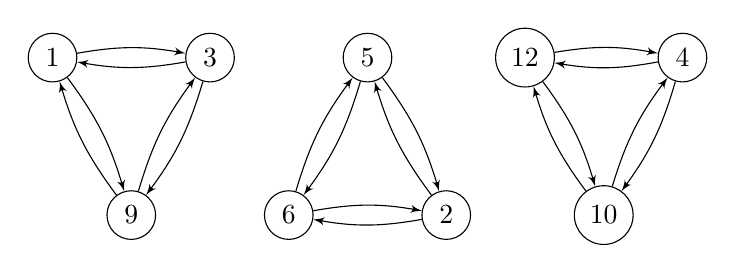
\begin{tikzpicture}
        
            \tikzset{vertex/.style = {shape=circle,draw,minimum size=1.5em}}	
            \tikzset{edge/.style = {->,> = latex'}}
            
	        \node[vertex] (n1) at (0,0) {$1$};
	        \node[vertex] (n3) at (2,0) {$3$};
	        \node[vertex] (n9) at (1,-2) {$9$};
	        
	        \node[vertex] (n6) at (3,-2) {$6$};
	        \node[vertex] (n2) at (5,-2) {$2$};
	        \node[vertex] (n5) at (4,0) {$5$};

	        \node[vertex] (n12) at (6,0) {$12$};
	        \node[vertex] (n4)  at (8,0) {$4$};
	        \node[vertex] (n10) at (7,-2) {$10$};
	        
	        \draw[edge] (n1) to [bend left=10] (n3);
	        \draw[edge] (n1) to [bend left=10] (n9);
	        \draw[edge] (n3) to [bend left=10] (n1);
	        \draw[edge] (n3) to [bend left=10] (n9);
	        \draw[edge] (n9) to [bend left=10] (n1);
	        \draw[edge] (n9) to [bend left=10] (n3);
	        
	        \draw[edge] (n2) to [bend left=10] (n5);
	        \draw[edge] (n2) to [bend left=10] (n6);
	        \draw[edge] (n5) to [bend left=10] (n2);
	        \draw[edge] (n5) to [bend left=10] (n6);
	        \draw[edge] (n6) to [bend left=10] (n2);
	        \draw[edge] (n6) to [bend left=10] (n5);
	        
	        \draw[edge] (n4) to [bend left=10] (n10);
	        \draw[edge] (n4) to [bend left=10] (n12);
	        \draw[edge] (n10) to [bend left=10] (n4);
	        \draw[edge] (n10) to [bend left=10] (n12);
	        \draw[edge] (n12) to [bend left=10] (n4);
	        \draw[edge] (n12) to [bend left=10] (n10);
	
	        %\draw[red, dashed] (1, 2) -- (1, -2);
	            
        \end{tikzpicture}
        \end{center}
    \end{frame}
    
     \begin{frame}
        Color the edges with $t$ distinct colors to differenciate recovering sets. \pause \\~\\
        
        Let $F$ be a coloring function of the edges:
        $$
            \begin{array}{ccccc}
                F: & E(G) & \longrightarrow & [t]  & \\
                   &(i,j) & \longmapsto     & \ell & \mbox{iff } j \in \R_i^\ell
            \end{array}
        $$ \pause \\~\\
        
    Remark: the out-degree of any vertex $i \in V$ is $\sum_\ell \vert \R_i^\ell \vert = tr$, and the edges leaving $i$ are colored in $t$ colors.
    
    \end{frame}    
    
    \begin{frame}
    Recovery graph for the $(12,4,\{2,3\})$-LRC code with edge coloring.
    
    Recall: 
    
    $\mathcal{A} = \left\lbrace  \left\lbrace 1, 5, 12 , 8 \right\rbrace, \left\lbrace 2 , 10 , 11 , 3 \right\rbrace , \left\lbrace 4 , 7 , 9 , 6 \right\rbrace \right\rbrace$
        
     $\mathcal{A'} = \left\lbrace  \left\lbrace 1 , 3 , 9 \right\rbrace, \left\lbrace 2 , 6 , 5 \right\rbrace , \left\lbrace 4 , 12 , 10 \right\rbrace , \left\lbrace 7 , 8 , 11 \right\rbrace \right\rbrace$
     \begin{center}
        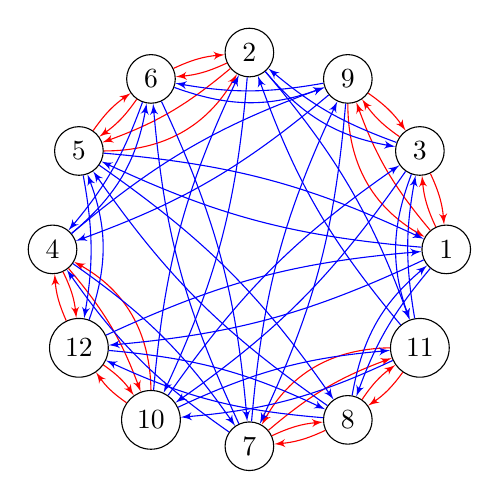
\begin{tikzpicture}
            \tikzset{vertex/.style = {shape=circle,draw,minimum size=1.5em}}	
            \tikzset{edge/.style = {->,> = latex',red}}
            \tikzset{edge2/.style = {->,> = latex',blue}}
            
            \def \radius {2.5cm}
            \def \n {12}
            
	        \node[vertex] (n1) at ({360/\n * (0)}:\radius) {$1$};
	        \node[vertex] (n3) at ({360/\n * (1)}:\radius) {$3$};
	        \node[vertex] (n9) at ({360/\n * (2)}:\radius) {$9$};
	        
	        \node[vertex] (n2) at ({360/\n * (3)}:\radius) {$2$};
	        \node[vertex] (n6) at ({360/\n * (4)}:\radius) {$6$};
	        \node[vertex] (n5) at ({360/\n * (5)}:\radius) {$5$};
	        
	        \node[vertex] (n4) at ({360/\n * (6)}:\radius) {$4$};
	        \node[vertex] (n12)  at ({360/\n * (7)}:\radius) {$12$};
	        \node[vertex] (n10) at ({360/\n * (8)}:\radius) {$10$};
	        
	        \node[vertex] (n7) at ({360/\n * (9)}:\radius) {$7$};
	        \node[vertex] (n8)  at ({360/\n * (10)}:\radius) {$8$};
	        \node[vertex] (n11) at ({360/\n * (11)}:\radius) {$11$};
	        
	        \draw[edge] (n1) to [bend left=10] (n3);
	        \draw[edge] (n1) to [bend left=10] (n9);
	        \draw[edge] (n3) to [bend left=10] (n1);
	        \draw[edge] (n3) to [bend left=10] (n9);
	        \draw[edge] (n9) to [bend right=30] (n1);
	        \draw[edge] (n9) to [bend left=10] (n3);
	        
	        \draw[edge] (n2) to [bend left=10] (n5);
	        \draw[edge] (n2) to [bend left=10] (n6);
	        \draw[edge] (n5) to [bend right=30] (n2);
	        \draw[edge] (n5) to [bend left=10] (n6);
	        \draw[edge] (n6) to [bend left=10] (n2);
	        \draw[edge] (n6) to [bend left=10] (n5);
	        
	        \draw[edge] (n4) to [bend left=10] (n10);
	        \draw[edge] (n4) to [bend left=10] (n12);
	        \draw[edge] (n10) to [bend right=30] (n4);
	        \draw[edge] (n10) to [bend left=10] (n12);
	        \draw[edge] (n12) to [bend left=10] (n4);
	        \draw[edge] (n12) to [bend left=10] (n10);
	        
	        \draw[edge] (n7) to [bend left=10] (n8);
	        \draw[edge] (n7) to [bend left=10] (n11);
	        \draw[edge] (n8) to [bend left=10] (n7);
	        \draw[edge] (n8) to [bend left=10] (n11);
	        \draw[edge] (n11) to [bend left=10] (n8);
	        \draw[edge] (n11) to [bend right=30] (n7);
	        
	        \draw[edge2] (n1) to [bend left=10] (n5);
	        \draw[edge2] (n1) to [bend left=10] (n12);
	        \draw[edge2] (n1) to [bend right=10] (n8);
	        
	        \draw[edge2] (n5) to [bend left=10] (n1);
	        \draw[edge2] (n5) to [bend left=10] (n12);
	        \draw[edge2] (n5) to [bend left=10] (n8);
	        
	        \draw[edge2] (n12) to [bend right=20] (n5);
	        \draw[edge2] (n12) to [bend left=10] (n1);
	        \draw[edge2] (n12) to [bend left=10] (n8);
	        
	        \draw[edge2] (n8) to [bend left=10] (n5);
	        \draw[edge2] (n8) to [bend left=10] (n12);
	        \draw[edge2] (n8) to [bend left=20] (n1);
	        
	        
	        \draw[edge2] (n2) to [bend right=20] (n3);
	        \draw[edge2] (n2) to [bend left=10] (n10);
	        \draw[edge2] (n2) to [bend left=10] (n11);
	        
	        \draw[edge2] (n3) to [bend left=10] (n2);
	        \draw[edge2] (n3) to [bend left=10] (n10);
	        \draw[edge2] (n3) to [bend right=20] (n11);
	        
	        \draw[edge2] (n10) to [bend left=10] (n3);
	        \draw[edge2] (n10) to [bend left=10] (n2);
	        \draw[edge2] (n10) to [bend left=10] (n11);
	        
	        \draw[edge2] (n11) to [bend left=10] (n3);
	        \draw[edge2] (n11) to [bend left=10] (n10);
	        \draw[edge2] (n11) to [bend left=10] (n2);

	        
	        \draw[edge2] (n4) to [bend right=20] (n6);
	        \draw[edge2] (n4) to [bend left=10] (n7);
	        \draw[edge2] (n4) to [bend left=10] (n9);
	        
	        \draw[edge2] (n6) to [bend left=10] (n4);
	        \draw[edge2] (n6) to [bend left=10] (n7);
	        \draw[edge2] (n6) to [bend right=20] (n9);
	        
	        \draw[edge2] (n7) to [bend left=10] (n6);
	        \draw[edge2] (n7) to [bend left=10] (n4);
	        \draw[edge2] (n7) to [bend left=10] (n9);
	        
	        \draw[edge2] (n9) to [bend left=10] (n6);
	        \draw[edge2] (n9) to [bend left=10] (n7);
	        \draw[edge2] (n9) to [bend left=10] (n4);
	            
        \end{tikzpicture}
        \end{center}
    \end{frame}
    
    
    \begin{frame}
    Recovery graph for the $(12,4,\{2,3\})$-LRC code with edge coloring.
    
    Recall: 

    $
        \mathcal{A} = \left\lbrace
        \only<5>{\textcolor{blue}}{\left\lbrace 1, 5, 12 , 8 \right\rbrace},
        \only<6>{\textcolor{blue}}{\left\lbrace 2 , 10 , 11 , 3 \right\rbrace},
        \only<7>{\textcolor{blue}}{\left\lbrace 4 , 7 , 9 , 6 \right\rbrace}
        \right\rbrace
    $
    
     $ 
         \mathcal{A'} = \left\lbrace
         \only<1>{\textcolor{red}}{\left\lbrace 1 , 3 , 9 \right\rbrace},
         \only<2>{\textcolor{red}}{\left\lbrace 2 , 6 , 5 \right\rbrace},
         \only<3>{\textcolor{red}}{\left\lbrace 4 , 12 , 10 \right\rbrace},
         \only<4>{\textcolor{red}}{\left\lbrace 7 , 8 , 11 \right\rbrace}
         \right\rbrace
     $   
        \begin{center}
        \begin{tikzpicture}
            \tikzset{vertex/.style = {shape=circle,draw,minimum size=1.5em}}	
            \tikzset{edge1/.style = {-,> = latex',red}}
            \tikzset{edge2/.style = {-,> = latex',blue}}
            
            \def \radius {2.5cm}
            \def \n {12}
            
	        \node[vertex] (n1) at ({360/\n * (0)}:\radius) {$1$};
	        \node[vertex] (n3) at ({360/\n * (1)}:\radius) {$3$};
	        \node[vertex] (n9) at ({360/\n * (2)}:\radius) {$9$};
	        
	        \node[vertex] (n2) at ({360/\n * (3)}:\radius) {$2$};
	        \node[vertex] (n6) at ({360/\n * (4)}:\radius) {$6$};
	        \node[vertex] (n5) at ({360/\n * (5)}:\radius) {$5$};
	        
	        \node[vertex] (n4) at ({360/\n * (6)}:\radius) {$4$};
	        \node[vertex] (n12)  at ({360/\n * (7)}:\radius) {$12$};
	        \node[vertex] (n10) at ({360/\n * (8)}:\radius) {$10$};
	        
	        \node[vertex] (n7) at ({360/\n * (9)}:\radius) {$7$};
	        \node[vertex] (n8)  at ({360/\n * (10)}:\radius) {$8$};
	        \node[vertex] (n11) at ({360/\n * (11)}:\radius) {$11$};
	        
	        \only<1,8>{
	        \draw[edge1] (n1) to (n3);
	        \draw[edge1] (n1) to (n9);
	        \draw[edge1] (n3) to (n9);
	        }
	        
	        \only<2,8>{
	        \draw[edge1] (n2) to (n6);
	        \draw[edge1] (n2) to (n5);
	        \draw[edge1] (n5) to (n6);
	        }
	        
	        \only<3,8>{
	        \draw[edge1] (n4) to (n10);
	        \draw[edge1] (n4) to (n12);
	        \draw[edge1] (n12) to (n10);
	        }
	        
	        \only<4,8>{
	        \draw[edge1] (n7) to (n8);
	        \draw[edge1] (n7) to (n11);
	        \draw[edge1] (n8) to (n11);
	        }
	        
	        \only<5,8>{
	        \draw[edge2] (n1) to (n5);
	        \draw[edge2] (n1) to (n12);
	        \draw[edge2] (n1) to (n8);
	        \draw[edge2] (n5) to (n12);
	        \draw[edge2] (n5) to (n8);
	        \draw[edge2] (n8) to (n12);
	        }
	        
	        \only<6,8>{
	        \draw[edge2] (n2) to (n10);
	        \draw[edge2] (n2) to (n11);
	        \draw[edge2] (n2) to (n3);
	        \draw[edge2] (n10) to (n11);
	        \draw[edge2] (n10) to (n3);
	        \draw[edge2] (n11) to (n3);
	        }
	        
	        \only<7,8>{
	        \draw[edge2] (n4) to (n7);
	        \draw[edge2] (n4) to (n9);
	        \draw[edge2] (n4) to (n6);
	        \draw[edge2] (n7) to (n9);
	        \draw[edge2] (n7) to (n6);
	        \draw[edge2] (n9) to (n6);
	        }
	        
    \end{tikzpicture}
    \end{center}
\end{frame}

\subsection{Proof for the rate bound}
\begin{frame}{Proof for the rate bound}
To prove bound on max. rate:
\begin{enumerate}
    \item Construct set $U$ of coordinates that can be recovered from $\overline{U} := [n]\setminus U$.
    \item Compute lower bound on $\card{U}$ $ \quad \longrightarrow \quad $ upper bound on $\card{\overline{U}}$
    \item u. bound on $\card{\overline{U}}$ $\rightarrow$ u. bound on $k$ $\rightarrow$ u. bound on max. rate 
\end{enumerate}
\end{frame}
   
    
    \chapter{Work Plan}
\end{document}